\chapter{基于自动属性提示的零样本细胞核检测}

\section{研究背景}
在医学图像处理领域，苏木精和曙红（H＆E）染色图像的细胞核检测在生物医学研究和临床应用的各个领域中发挥着至关重要的作用\cite{gleason1992histologic}。进行像素级实例掩码的标注工作是极其费时费力的，需要医生重复标注大量细胞，并且由于细胞核往往密集和微小，比自然图像或者其他类型的医学图像数据集（比如眼底，骨骼，器官组织等）更加难以标注。像素级实例掩码还要求更精确的轮廓，相比之下，在传统细胞核检测场景中，模型如果依赖大量边界框或点级标注进行训练能相对降低标注成本，但在真实病理研究中，构建多数据集、多中心和多类别核检测标注依然代价高昂。尤其是在研究新组织类型、稀有类别或跨域迁移问题时，检测标注往往成为限制模型快速拓展的重要瓶颈。总之无论是采用何种形式的标注，其标注准备工作的繁杂程度都是难以承受的，极大得阻碍了相关的科学研究和技术应用。具体来说，比如\cite{mahanta2021ihc,graham2019hover,yi2019multi}等方法提出了完全监督的有效方法，但由于标注工作仍然是劳动密集型且昂贵的，现实应用中依然困难重重。

为了解决上述问题，人们提出了几种无监督方法，包括基于阈值保持的方法\cite{jiao2006improved,mouelhi2018fast}、基于自监督的方法\cite{sahasrabudhe2020self}和基于领域适应的方法\cite{le2022unsupervised}。其中，域适应方法是主流，通过对齐源域和目标域来实现适应，并表现出良好的性能\cite{le2022unsupervised}。然而，当前的无监督方法表现出较强的经验设计，使得在模型设计过程中引入了主观偏差，因此当前的无监督方法可能会导致次优结果。然而，新开发的大规模视觉语言预训练模型（VLPM）提供了另一种可能的无监督学习范式\cite{radford2021learning,jia2021scaling}。 VLPM 从互联网上获取的大量文本图像对中学习对齐的文本和图像特征，使学习到的视觉特征语义丰富、通用且可转移。基于VLPM的零样本学习方法用于文本驱动的图像处理\cite{patashnik2021styleclip}、图像字幕\cite{li2022blip}、视图合成\cite{jain2021putting}和目标检测\cite{li2022grounded}等下游任务，取得了优异的结果。在 VLPM 中，在对象级别进行预训练的基础语言图像预训练（GLIP）模型 \cite{li2022grounded} 甚至可以在零样本对象检测和短语基础任务中与完全监督的模型相媲美。尽管 VLPM 已被用于自然场景中的物体检测，但通过 VLPM 对 H\&E 图像进行零样本核检测仍然没有得到充分探索。医学 H\&E 图像与用于预训练的自然图像之间的显着域差异使得这项任务具有挑战性。人们想知道VLPM是否可以凭借其丰富的语义信息，通过语义驱动的提示来直接预测细胞核检测，建立一个优雅、简洁、清晰但更高效和可移植的无监督系统，用于无标记细胞核检测。基于这个概念，我们的目标是建立一个基于 VLPM 的零样本核检测框架。然而，直接应用 VLPM 来完成这项任务会带来两个挑战。 （1）由于医学图像和用于预训练的网络源文本图像对之间存在差距，文本编码器可能缺乏医学概念词的先验知识，从而使零样本检测的提示设计成为一项具有挑战性的任务。 (2)与自然图像中的物体不同，H\&E染色图像中细胞核的高密度和特殊形态可能会导致在零样本传输过程中仅根据提示进行漏检、误检和重叠。为了解决第一个挑战，Yamada 等人分析发现，在大量文本-图像对的预训练下，无论图像域如何，VLPM 在对象与其语义属性之间建立了强关联绑定，即关联属性文本可以通过 VLPM 完整地描述图像中对应的对象\cite{yamada2022lemons}。因此，VLPM通过构建适当的模型以无标签的方式检测未见过的医学对象（即细胞核这类具体物体）是可行的。
理论上只需提供目标文本描述，就能够在新图像中定位相关对象。然而，这种能力在医学图像中并不能无缝成立。病理图像中的“细胞核”“浆细胞”“中性粒细胞”一类概念，不仅在视觉形态上细粒度差异大，而且在通用预训练语料中也并不总能得到充分覆盖。因此，如何让视觉语言模型在医学场景中真正发挥零样本检测能力，成为本章的核心问题。
虽然可以通过人工手动编写提示词来让VLPM认识到目标细胞核的特征，但手动提示是一个繁琐且主观的过程，可能会导致相当大的偏见。然而，VLPM 网络 BLIP \cite{li2022blip} 具有生成图像自动描述的能力。因此，我们首先使用BLIP自动生成属性词来描述看不见的细胞核对象。这种方法避免了经验性的手动提示设计，并充分利用了 VLPM 的文本到图像对齐特性。随后，我们将这些属性词与医学名词相结合，即“[形状][颜色][名词]”，以创建检测提示。然后将这些提示输入GLIP中，实现原子核的零射击检测。我们提出的自动提示设计方法充分利用了VLPM的文本到图像对齐，并能够自动生成描述相应领域的最合适的属性文本单词。我们的方法提供了出色的可解释性。通过GLIP强大的对象检索性能，我们可以获得初步的框。这些初步框的精度相对较高，但召回率仍有相当大的提升空间。因此，我们进一步建立了一个自我训练框架。我们使用 GLIP 生成的初步框作为伪标签来进一步训练 YOLOX \cite{ge2021yolox}，以迭代方式细化和完善预测框。与自我训练策略相结合，所得模型在无标记细胞核检测方面取得了显着的性能，超越了其他比较方法。我们证明，在自然图像文本对上进行预训练的 VLPM 在医学领域的下游任务中也表现出惊人的潜力。本文的贡献有三个方面。 (1)提出了一种基于VLPM的新型零样本无标签核检测框架。我们的方法执行所有现有的无监督方法，并表现出出色的可移植性。 （2）我们利用GLIP，与对比语言图像预训练（CLIP）模型相比，GLIP更强调对象级表示学习并生成更高质量的语言感知视觉表示，以实现更好的核检索。 (3)基于VLPM的关联结合特征建立自动提示设计过程，以避免繁琐的经验手动提示工程。

\section{问题定义}
本章关注的任务是：在没有目标域检测标注、甚至没有明确人工医学 prompt 模板的条件下，实现对细胞核目标的零样本检测。具体而言，给定一张病理图像，模型需要输出可能的目标位置，而训练阶段不能依赖专门为该检测任务构建的大量框标注。

这一问题可以进一步拆解为两个层次。第一，模型必须首先“理解”目标，即把医学对象的视觉特征与语义描述连接起来。第二，模型还需要把这种粗粒度理解转化为稳定的目标定位能力。前者是提示构造问题，后者是性能适配问题。本文围绕这两个层次设计了自动属性提示与自训练联合框架。

\section{研究动机}
如果直接将简单的医学类名作为文本提示，例如仅使用“nucleus”或“tumor nucleus”，模型通常难以稳定聚焦于真正目标区域。原因在于这类词汇过于抽象，无法提供足够细粒度的外观线索。在自然图像任务中，“dog”“car”等类名往往已足够区分类别，但在医学图像中，相邻细胞类别之间的差异可能只体现在细微形态、颜色深浅或局部纹理上。纯粹依赖类名的文本提示，往往不足以唤起模型对这些差异的敏感性。

因此，本章的一个核心动机是：不能把 prompt 仅仅理解为“类别名称字符串”，而应将其理解为“帮助模型建立目标语义入口的描述载体”。在医学场景中，这个载体理应包括更多属性信息，例如核形态、染色表现、周围背景关系等。基于这一认识，本章提出自动属性提示构造策略，使 prompt 从静态类名升级为更具辨识力的语义组合。

\section{方法总体框架}
本章方法由三个核心步骤组成。第一步，自动生成与目标相关的属性描述。第二步，将这些属性与类别名称或任务描述组合成用于视觉语言检测器的文本提示。第三步，在获得初始零样本预测后，以高置信结果作为伪标签，对模型进行自训练或再适配。

这一设计使模型的知识来源发生了变化：它不再完全依赖人工标注数据，而是部分依赖于视觉语言预训练带来的跨模态先验，以及自动构造的属性语义信息。进一步地，自训练步骤又让模型可以从目标域图像本身反向吸收知识，实现从“开放词汇泛化”到“目标域适配”的过渡。

\section{自动属性提示构造}
\subsection{使用对象级视觉语言大模型GLIP的优势}
近年来，诸如 CLIP \cite{radford2021learning} 和 ALIGN \cite{jia2021scaling} 之类的大型 VLPM 在通用视觉表示学习方面取得了巨大进展，并展示了利用提示进行零样本迁移的巨大潜力。典型的 VLPM 框架包含两个编码器：文本编码器，将文本提示编码为语义丰富的文本嵌入，以及图像编码器，它将图像编码为视觉嵌入。这些 VLPM 使用大量源自网络的文本图像对 {(X, T)}i 通过文本和视觉嵌入的对比损失来学习文本到图像的对齐。将图像编码器表示为 EI，文本编码器表示为 ET，余弦相似度函数表示为 cos(·)，并假设每个训练时期使用 K 个文本图像对，对比学习的目标可以表示为：

\begin{equation}
\label{eq:contrastive}
\mathcal{L}_c=-\sum_{i=1}^K \log \frac{\exp \left(\cos \left(E_I\left(X_i\right), E_T\left(T_i\right)\right) / \tau\right)}{\sum_{j=1}^K \exp \left(\cos \left(E_I\left(X_i\right), E_T\left(T_j\right)\right) / \tau\right)}.
\end{equation}

通过这种对齐对比学习，VLPM 在公共特征空间中对齐文本和图像，允许人们通过操作文本（即提示工程）将经过训练的 VLPM 直接传输到下游任务。借助对齐的文本图像对，输入图像的视觉表示语义丰富且易于解释。然而，传统的VLPM预训练过程仅从整体角度将图像与文本对齐，这导致缺乏对对象级表示的重视。因此，李等人。提出了 GLIP \cite{li2022grounded}，其图像编码器为图像中不同区域的每个对象生成视觉嵌入，以与文本中存在的对象词对齐。此外，GLIP 利用基于网络的短语基础文本图像对来提取新的对象词实体，扩展了文本编码器中的对象概念。此外，与仅在模型末尾对齐嵌入的 CLIP 不同，GLIP 利用交叉注意力机制构建了一个深度跨模态融合模块\cite{chen2021crossvit}，用于多级对齐，这样能够使得多级结构中每一级都进行了高度对齐，比只在一个最终特征空间进行对齐要更加稳定可靠。如图1（a）所示，GLIP分别利用DyheadModules \cite{dai2021dynamic}和BERTLayer \cite{devlin2018bert}作为图像和文本编码层。将文本嵌入表示为 $R$，视觉嵌入表示为 $P$，深度融合过程可以表示为：

\begin{equation}
\label{eq:glip_xmha}
R_{\mathrm{t}2\mathrm{i}}^{i}, P_{\mathrm{i}2\mathrm{t}}^{i}=\mathrm{X\text{-}MHA}\left(R^{i}, P^{i}\right),\quad i \in\{0,1, \ldots, L-1\}.
\end{equation}
\begin{equation}
\label{eq:glip_dyhead}
R^{i+1}=\mathrm{DyHeadModule}\left(R^{i}+R_{\mathrm{t}2\mathrm{i}}^{i}\right),\quad \cdots\quad R=R^{L}.
\end{equation}
\begin{equation}
\label{eq:glip_bert}
P^{i+1}=\mathrm{BERTLayer}\left(P^{i}+P_{\mathrm{i}2\mathrm{t}}^{i}\right),\quad \cdots\quad P=P^{L}.
\end{equation}

其中L是总层数，R0表示来自swin Transformer-large \cite{liu2021swin}的视觉特征，P 0 表示来自BERT \cite{devlin2018bert}的标记特征。 X MHA 代表交叉注意力。该架构使 GLIP 能够获得卓越的对象级性能和语义聚合。因此，GLIP 比传统 VLPM 更适合对象级零样本传输。因此，我们采用 GLIP 来提取更好的对象级表示以进行核检测。

\subsection{自动构造提示词}
文本输入（称为提示）在 VLPM 向下游任务的零样本传输中起着至关重要的作用。 GLIP最初使用连接的对象名词如“对象名词1.对象名词2...”作为默认的检测文本提示，并且还允许手动工程以提高性能\cite{li2022grounded}。然而，手动提示工程是一项不小的挑战，需要大量的努力和专业知识。此外，源自网络的预训练文本图像对和医学图像之间存在显着的差异。因此，简单的名词串联不足以让 GLIP 识别到目标细胞核。如果完全依赖研究者手写属性短语，方法虽然可行，但很难扩展到新的数据集、新的目标或新的组织场景。本章强调“自动属性提示”的一个重要原因，就是希望让 prompt 构造过程尽量摆脱人工模板工程的限制。这样，当任务从某一病理场景迁移到另一病理场景时，系统可以通过自动描述和重新组合属性，快速构造新的目标提示。
在医学病理图像中，一个类别的判别性常常不只来自类别名，而来自其属性组合。例如，同为免疫细胞，不同亚型在大小、核质比、染色均匀性和轮廓规则性上可能存在细微差别。若这些差异无法被文本提示显式反映，视觉语言模型就难以可靠地区分类别。因此，将属性信息引入 prompt，是从通用视觉语言模型向医学检测器迁移的关键一步。

我们注意到山田等人。证明对大量文本图像对的预训练使得 VLPM 能够在对象及其语义属性之间建立强大的关联绑定\cite{yamada2022lemons}。因此，通过VLPM，关联的属性文本可以准确地描述相应的对象。基于这项研究，我们提出 VLPM 有潜力通过构建相关属性文本以零样本的方式检测未标记的医疗对象。如图1（a）所示，我们首先使用图像描述VLPM BLIP \cite{li2022blip}自动生成属性词来描述看不见的核对象。 BLIP 使我们能够避免手动属性设计并生成符合 VLPM 文本到图像对齐的属性语音表。这个过程涉及三个步骤。 （1）直接将目标医学名词输入GLIP进行粗框预测。 (2)使用粗框对图像进行方形裁剪，将裁剪后的对象输入到冻结的BLIP中，以自动生成描述对象的属性词。 (3)通过词频统计和分类，分别找出描述物体形状和颜色的前M个词，因为“形状”和“颜色”是描述物体核最相关的两个属性。为了获得完整的描述，我们使用预先训练的语言模型检索到的同义词来扩充属性词\cite{radford2019language}。

结合那些医学名词，自动生成“[形状][颜色][名词]”的三联体检测提示。最后，所有生成的三元组都放入 GLIP 中进行精细检测。该方法避免了经验性的手动提示设计，充分利用了VLPM的文本到图像对齐特性。我们的自动提示设计利用了 GLIP 和 BLIP 强大的文本到图像对齐功能。这种方法还能够自动生成针对特定领域的最合适的属性词，体现了出色的可解释性。

在检测器内部，属性提示并不是孤立存在的文字片段，而是与类别语义共同构成查询条件。它的作用可以理解为对类名进行细化和约束，使视觉语言模型不仅知道“目标是什么”，还知道“它通常具备哪些视觉特征”。这种提示方式对零样本场景尤其有意义，因为它增强了模型在缺乏显式监督时的判别依据。

\section{视觉语言零样本检测器}
在得到属性提示后，本章将其输入视觉语言预训练检测器进行零样本推理。与传统闭集检测器不同，这里的检测器在预训练时已经学到图文对齐知识，因此具有一定开放词汇迁移能力。其优势在于：即使没有在目标域上进行大规模监督训练，也能通过语义提示给出一定质量的初始候选框。

然而，这种初始预测通常存在两个常见问题。其一，召回率有限，许多难例会被漏检。其二，定位稳定性不够，尤其在病理图像这类高密度细粒度场景中，候选框容易偏移或碎裂。因此，本章并不把零样本预测视为终点，而是把它当作后续自训练的起点。

\section{自训练与目标域适配}
利用GLIP强大的目标检索性能，我们获得了高精度但召回率较低的初步检测框。这些框存在漏检、误检和重叠等问题。为了充分发挥 GLIP 的零样本潜力，建立了一个自我训练框架。自动提示被输入到 GLIP 中以生成初始结果，作为训练 YOLOX 的伪标签 \cite{ge2021yolox}。然后，以融合后的YOLOX为教师生成新的伪标签，并迭代训练学生YOLOX。由于自我训练基于 EM 优化算法 \cite{moon1996expectation}，它推动我们的系统不断细化预测框并实现更好的优化。
视觉语言模型提供的是一种通用语义入口，但目标域性能往往仍需要进一步适配。自训练在这里扮演的角色，不是替代零样本能力，而是将其转化为目标域内部更可用的检测性能。通过筛选高置信候选框并迭代更新模型，检测器可以逐步对目标域的外观分布、目标尺度和背景噪声形成更稳定认识。
伪标签在本章中具有双重作用。一方面，它是零样本检测结果向监督训练结果过渡的桥梁；另一方面，它也起到筛选和浓缩目标域信息的作用。通过适当的置信度控制和更新策略，伪标签能帮助模型聚焦于更可靠的目标实例，从而减少开放词汇模型直接迁移时的噪声。

\begin{figure}[H]
  \centering
  % 原图来自论文工程（PAPERS/glip\_miccai\_camera\_ready\_version）
  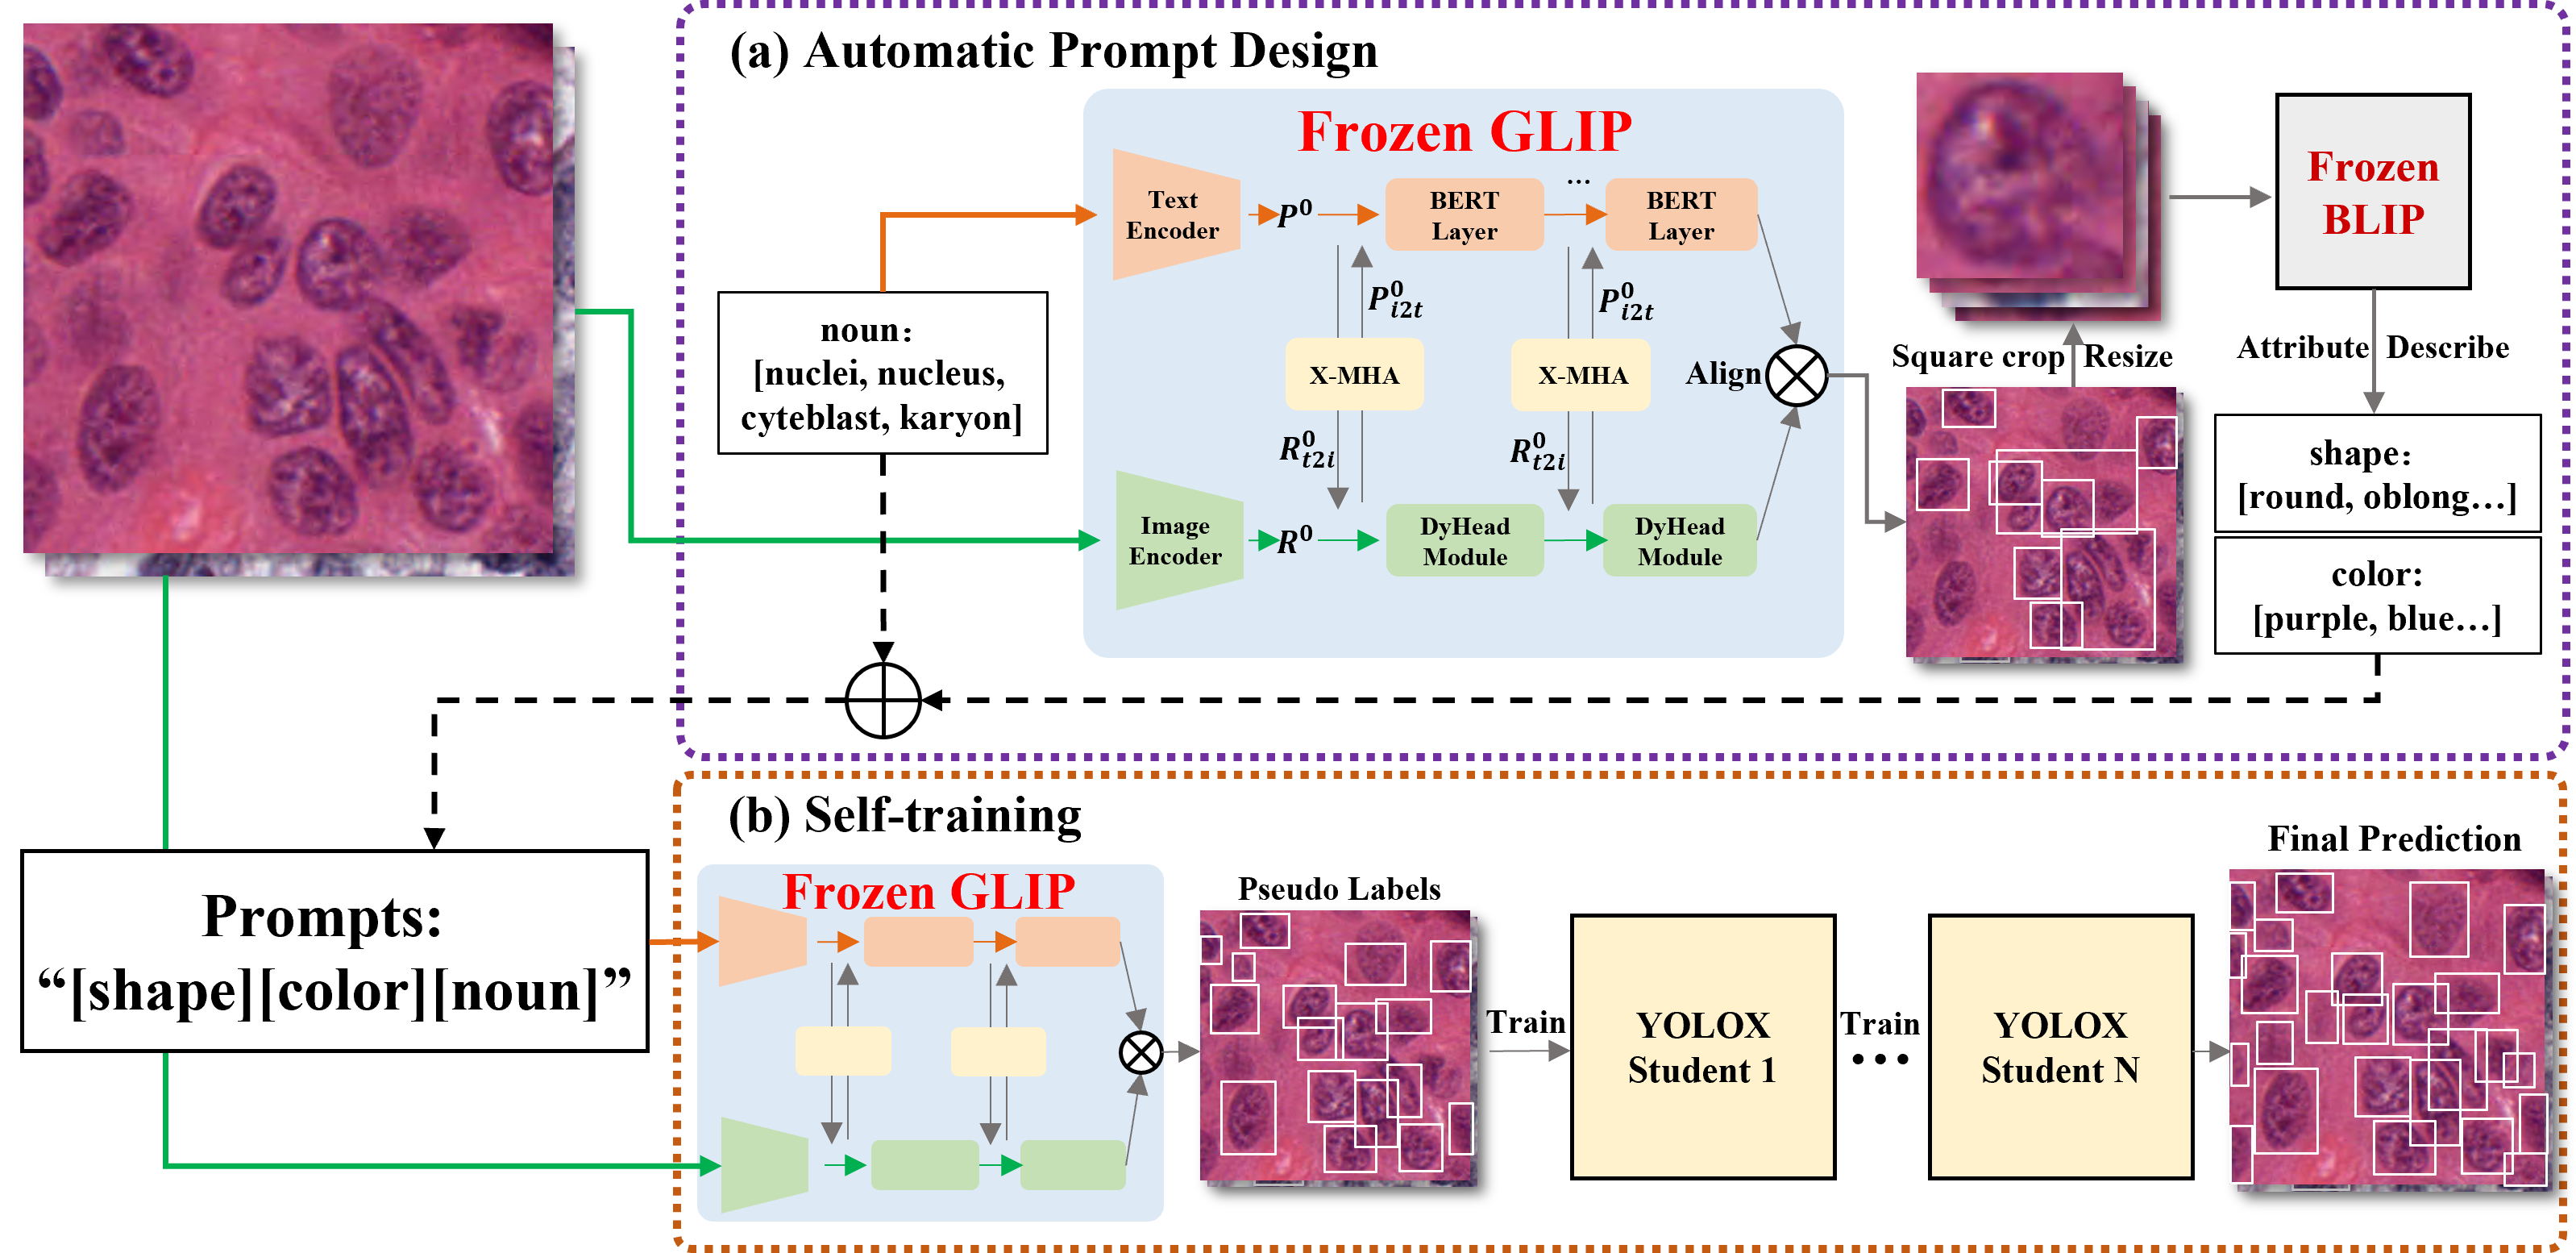
\includegraphics[width=\textwidth]{chapters/PAPERS/glip_miccai_camera_ready_version/paper2592_method.png}
  \caption{基于对象级视觉语言预训练模型 GLIP 的零样本细胞核检测框架。(a) 给定任务的目标医学名词后，基于视觉语言模型的语义属性关联特性以及图像到文本模型 BLIP，自动构造属性提示词，避免繁琐且主观的手工 prompt 工程；(b) 进一步引入自训练策略，以 GLIP 的初始预测作为伪标签，迭代训练检测器以提升召回率与定位质量。}
  \label{fig:zeroshot_framework}
\end{figure}
图 \ref{fig:zeroshot_framework} 展示了本章方法从“自动属性构造”到“零样本检测”再到“目标域自训练”的完整流程。自动属性提示的作用在于增强类名的辨识能力，使模型不再只根据粗粒度类别词汇进行定位；自训练阶段则把初始零样本预测转化为可持续优化的伪监督信号，使模型逐步吸收目标域视觉统计特征。这样的设计既延续了视觉语言模型的开放词汇能力，也兼顾了医学检测任务对稳定性的要求。

\section{实验设计}
\subsection{数据集准备}
本研究使用的数据集是MoNuSeg数据集\cite{kumar2017dataset}，它由30张大小为1000×1000的细胞核图像组成，平均每张图像有658个细胞核。继库马尔等人之后\cite{kumar2017dataset}，数据集被分成训练集和测试集，比例为16:14。 16 张训练图像作为 GLIP 的输入，生成用于自我训练的伪标签，并随机选择 4 张图像进行验证。注释仅用于测试图像的评估目的。从每个图像中提取 16 个大小为 256 × 256 的重叠图像块，并随机裁剪为 224 × 224 作为输入。在实验设置方面，使用了四个 Nvidia RTX 3090 GPU，每个 GPU 具有 24 GB 内存。在自动提示生成过程中，使用在ViT-B和CapFilt-L \cite{li2022blip}上微调的BLIP的VQA权重来生成[形状]和[颜色]属性。这些属性词通过 GPT \cite{radford2019language} 用同义词进行增强，即属性增强。目标医学名词列表首先直接设置为[“nuclei”]，并通过GPT扩充为[“nuclei”、“nucleus”、“cyteblast”、“karyon”]，即名词扩充。随后将属性词与目标医学名词组合成“[形状][颜色][名词]”格式作为 GLIP 的输入，生成边界框作为伪标签。 GLIP 使用的权重是 GLIP-L。对于自我训练细化，我们使用 YOLOX 的默认设置并遵循\cite{dopido2013semisupervised}中描述的标准自我训练方法。

\begin{table}[htbp]
  \centering
  \caption{MoNuSeg \cite{kumar2017dataset} 上的对比结果。无监督方法的最佳结果以粗体标记。}
  \label{tab:zeroshot_comparison}
  \begin{tabular}{c|c|cccc}
    \hline
    \textbf{supervision} & \textbf{method} & \textbf{mAP} & \textbf{AP50} & \textbf{AP75} & \textbf{AR} \\ \hline
    \textbf{fully-supervised} & \textbf{YOLOX (2021)} & 0.447 & 0.832 & 0.437 & 0.528 \\ \hline
    \multirow{4}{*}{\textbf{unsupervised}} & \textbf{SSNS (2020)} & 0.354 & 0.739 & 0.288 & 0.441 \\
     & \textbf{SOP (2022)} & 0.235 & 0.609 & 0.096 & 0.351 \\
     & \textbf{VLDet (2023)} & 0.173 & 0.407 & 0.112 & 0.263 \\
     & \textbf{Ours} & \textbf{0.416} & \textbf{0.808} & \textbf{0.382} & \textbf{0.502} \\ \hline
  \end{tabular}
\end{table}

\subsection{主结果与对比实验}
我们将所提出的基于 GLIP 的零样本核检测方法，与全监督检测器 YOLOX \cite{ge2021yolox} 以及代表性的无监督/零样本检测方法进行对比，包括 SSNS \cite{sahasrabudhe2020self}、SOP \cite{le2022unsupervised} 和 VLDet \cite{lin2022learning}。评估指标遵循 COCO \cite{lin2014microsoft}，报告 mAP、AP50、AP75 与 AR（召回率）。如表 \ref{tab:zeroshot_comparison} 所示，在不使用任何目标域框标注的条件下，本文方法在 mAP 与 AP50 等指标上显著优于现有无监督基线，并在整体性能上逼近全监督 YOLOX 的结果。

\begin{figure}[H]
  \centering
  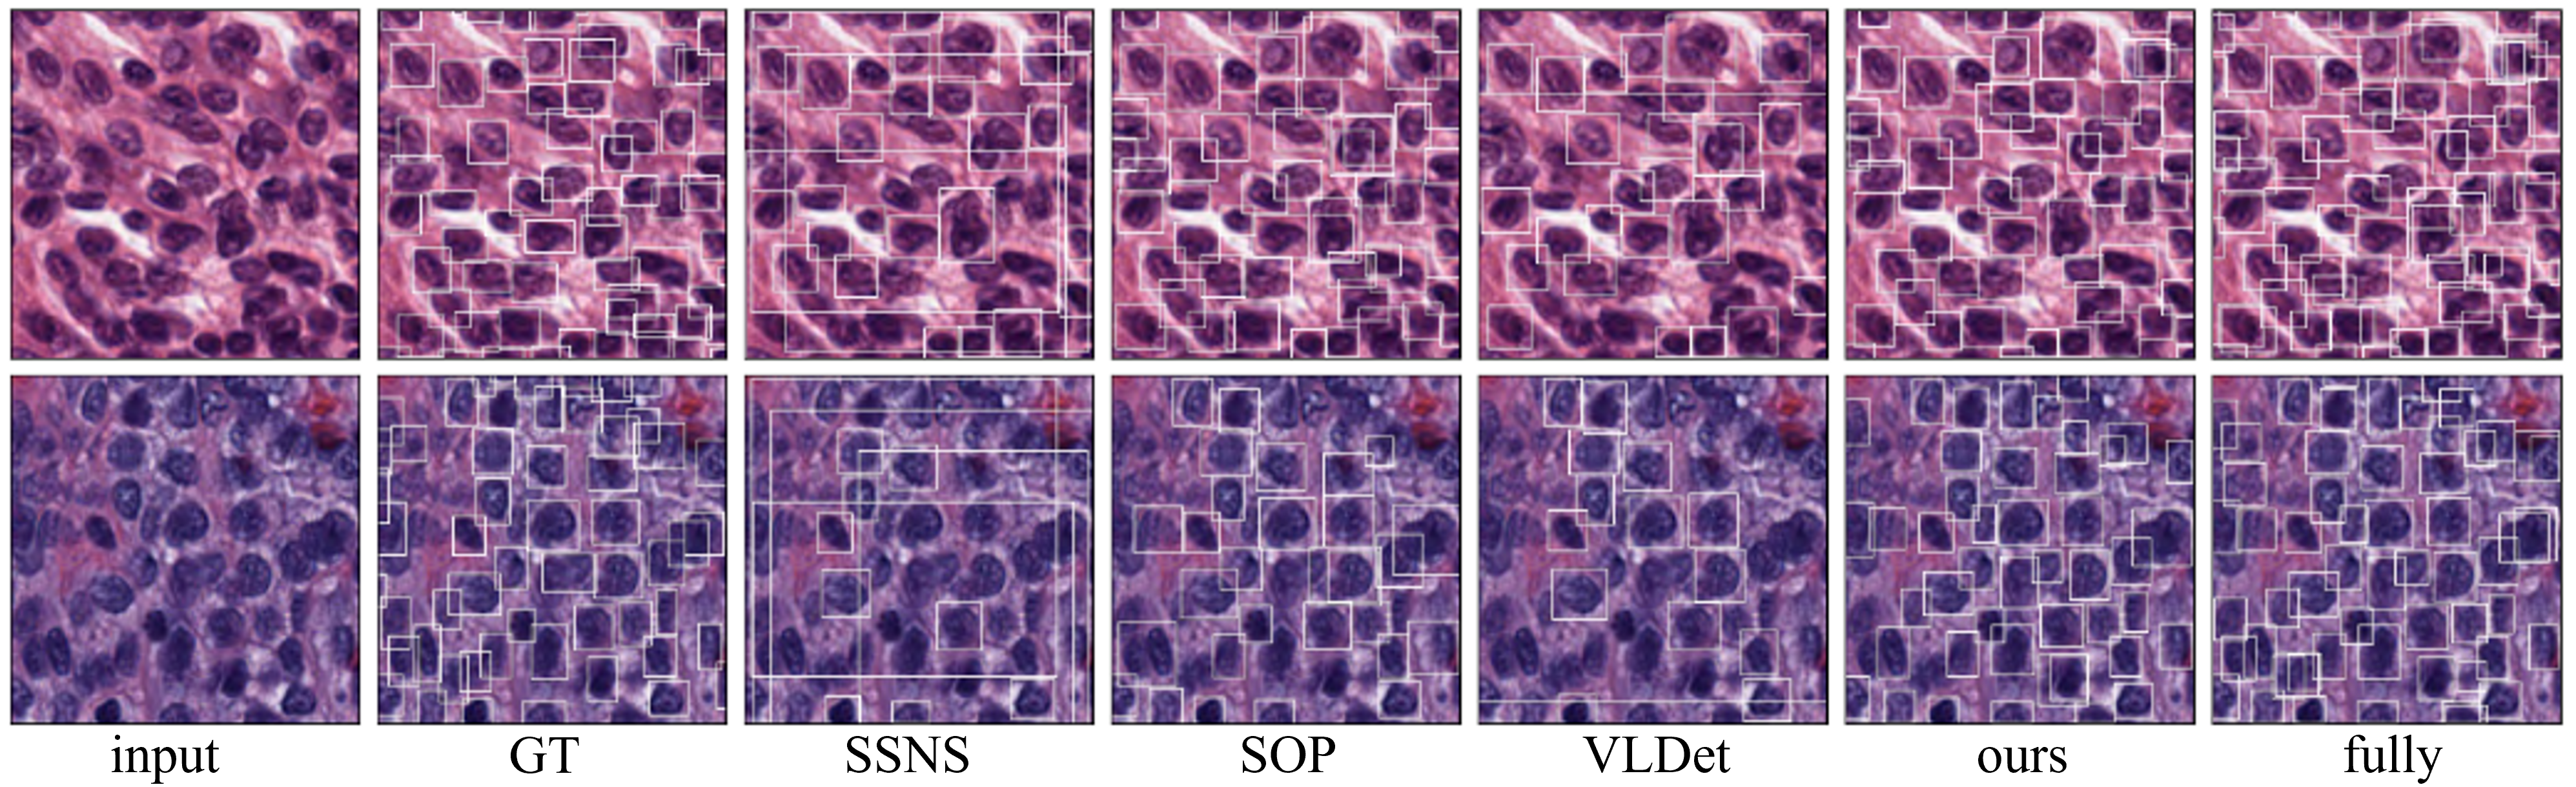
\includegraphics[width=\textwidth]{chapters/PAPERS/glip_miccai_camera_ready_version/paper2592_comparison.png}
  \caption{不同方法的检测结果可视化对比。图中白色边界框为模型预测结果，可用于观察零样本提示与自训练适配在召回率与定位质量上的差异。}
  \label{fig:zeroshot_vis}
\end{figure}

\subsection{消融实验}
\subsubsection{自动提示（prompt）构造策略}
我们首先针对 prompt 设计做消融实验，在其余设置保持一致（均使用相同的自训练流程直至收敛）的情况下对比不同提示形式，结果如表 \ref{tab:zeroshot_prompt} 所示。可以看到，仅使用医学名词串联（\textbf{noun}）时性能极差（mAP=0.064），说明医学名词与通用预训练语料之间的概念鸿沟会显著阻碍 VLPM 的直接零样本迁移。加入人工属性描述（\textbf{manual design}）后，性能大幅提升，验证了“属性描述”对核检索的重要性；但人工撰写具有经验性与主观性，难以在不同组织/染色/中心间稳定泛化。

与人工提示相比，自动提示生成能够在无模板、无人工先验的条件下生成可解释的属性词组合。进一步观察表 \ref{tab:zeroshot_prompt} 的后四行：当 prompt 从仅包含单一属性（shape 或 color）逐步扩展为同时包含形状与颜色，再结合名词形成三联体 \textbf{[shape][color][noun]} 时，检测性能呈现持续上升趋势。尤其值得注意的是，\textbf{auto: [shape][color]} 在不显式包含名词的情况下也能取得较强结果，说明 BLIP 自动生成的属性词本身已能有效刻画“核”这一目标的典型外观。

\begin{table}[htbp]
  \centering
  \renewcommand{\arraystretch}{1.1}
  \caption{不同 prompt 构造策略的消融结果（最后 4 行为自动生成提示）。最佳结果以粗体标记。}
  \label{tab:zeroshot_prompt}
  \begin{tabular}{l|rrrr}
    \hline
    \textbf{prompt design} & \textbf{mAP} & \textbf{AP50} & \textbf{AP75} & \textbf{AR} \\ \hline
    \textbf{noun} & 0.064 & 0.152 & 0.036 & 0.150 \\
    \textbf{manual design} & 0.414 & 0.757 & 0.422 & \textbf{0.509} \\ \hline
    \textbf{auto: [shape][noun]} & 0.336 & 0.604 & 0.350 & 0.434 \\
    \textbf{auto: [color][noun]} & 0.213 & 0.447 & 0.176 & 0.325 \\
    \textbf{auto: [shape][color]} & 0.413 & 0.726 & \textbf{0.438} & 0.498 \\
    \textbf{auto: [shape][color][noun]} & \textbf{0.416} & \textbf{0.808} & 0.382 & 0.502 \\ \hline
  \end{tabular}
\end{table}

\subsubsection{词汇增强（augmentation）策略}
我们进一步分析属性/名词增强对性能的影响，如表 \ref{tab:zeroshot_aug} 所示。其中，属性增强（A Aug.）通过同义词扩展形状与颜色属性；名词增强（N Aug.）将名词列表从 [``nuclei''] 扩展为 [``nuclei'', ``nucleus'', ``cyteblast'', ``karyon'']。实验表明：属性增强整体有效；而名词增强反而可能带来性能下降。其原因在于扩展得到的同义医学名词更偏“低频术语”，在 GLIP 的通用预训练语料中出现概率更低，导致提示词对齐质量下降。相对地，属性词多为自然语言中常见的外观描述，更符合 VLPM 的预训练分布，因此更稳定。

\begin{table}[htbp]
  \centering
  \renewcommand{\arraystretch}{1.1}
  \caption{词汇增强策略消融实验结果。其中 ``A Aug.'' 与 ``N Aug.'' 分别表示属性增强（attribute augmentation）与名词增强（noun augmentation）。}
  \label{tab:zeroshot_aug}
  \begin{tabular}{c|c|cccc}
    \hline
    \textbf{A Aug.} & \textbf{N Aug.} & \textbf{mAP} & \textbf{AP50} & \textbf{AP75} & \textbf{AR} \\ \hline
     &  & 0.372 & 0.725 & 0.337 & 0.464 \\
    \checkmark &  & \textbf{0.416} & \textbf{0.808} & \textbf{0.382} & \textbf{0.502} \\
     & \checkmark & 0.316 & 0.754 & 0.182 & 0.419 \\
    \checkmark & \checkmark & 0.332 & 0.659 & 0.296 & 0.434 \\ \hline
  \end{tabular}
\end{table}

\subsubsection{自训练过程与伪标签质量分析}
自训练阶段的核心作用是：将 GLIP 的初始高精度候选框转化为更高召回、更稳定的目标域检测器。表 \ref{tab:zeroshot_selftrain} 汇报了从原始 GLIP 教师（T0）到多轮 YOLOX 学生（S1--S5）的性能演化。可以观察到：原始 GLIP 的精度较高（Precision=0.678），但召回不足（Recall=0.310）；随着自训练迭代进行，召回与整体 mAP 持续提升并趋于收敛，最终达到本文的最佳配置（S4，对应表 \ref{tab:zeroshot_comparison} 的 Ours）。图 \ref{fig:miccai_selftrain} 给出了不同阶段的可视化对比。

\begin{table}[htbp]
  \centering
  \renewcommand{\arraystretch}{1.1}
  \caption{自训练策略有效性分析（IoU=0.5 下计算 Precision/Recall）。T 表示教师，S 表示学生。最佳结果以粗体标记。}
  \label{tab:zeroshot_selftrain}
  \begin{tabular}{c|cc|cccc}
    \hline
    \textbf{T/S} & \textbf{Precision} & \textbf{Recall} & \textbf{mAP} & \textbf{AP50} & \textbf{AP75} & \textbf{AR} \\ \hline
    \textbf{Raw GLIP T0} & 0.678 & 0.310 & 0.146 & 0.252 & 0.165 & 0.213 \\
    \textbf{YOLOX S1} & 0.733 & 0.706 & 0.293 & 0.636 & 0.224 & 0.397 \\
    \textbf{YOLOX S2} & 0.807 & 0.754 & 0.359 & 0.698 & 0.335 & 0.445 \\
    \textbf{YOLOX S3} & \textbf{0.814} & 0.815 & 0.404 & 0.755 & 0.395 & 0.497 \\
    \textbf{YOLOX S4} & 0.813 & \textbf{0.820} & \textbf{0.416} & \textbf{0.808} & 0.382 & 0.502 \\
    \textbf{YOLOX S5} & \textbf{0.814} & 0.807 & 0.414 & 0.742 & \textbf{0.436} & \textbf{0.509} \\ \hline
  \end{tabular}
\end{table}

为了验证“性能提升来自 VLPM 的语义伪标签，而非仅来自 YOLOX 或自训练技巧”，我们进一步用一种常见的无监督目标生成方法（超像素）替代 GLIP 生成伪标签，并保持相同自训练设置。结果如表 \ref{tab:zeroshot_superpixel} 所示，整体性能显著落后，说明高质量的零样本伪标签生成是方法成立的关键。

\begin{table}[htbp]
  \centering
  \renewcommand{\arraystretch}{1.1}
  \caption{用超像素方法生成伪标签并进行同样自训练的结果（对比说明 VLPM 伪标签的重要性）。}
  \label{tab:zeroshot_superpixel}
  \begin{tabular}{c|cccc}
    \hline
    \textbf{T/S} & \textbf{mAP} & \textbf{AP50} & \textbf{AP75} & \textbf{AR} \\ \hline
    \textbf{Superpixels T0} & 0.027 & 0.075 & 0.012 & 0.035 \\
    \textbf{YOLOX S1} & 0.260 & 0.612 & 0.162 & 0.373 \\
    \textbf{YOLOX S2} & 0.272 & 0.617 & 0.183 & 0.392 \\
    \textbf{YOLOX S3} & \textbf{0.284} & \textbf{0.655} & 0.169 & \textbf{0.404} \\
    \textbf{YOLOX S4} & 0.279 & 0.614 & \textbf{0.213} & 0.389 \\ \hline
  \end{tabular}
\end{table}

此外，我们也测试将自训练检测架构从 YOLOX 替换为 DETR \cite{carion2020end} 的可行性。如表 \ref{tab:zeroshot_detr} 所示，替换后性能仍保持在较高水平，说明方法的关键在于“语义驱动的伪标签生成”，而非强依赖某一特定检测器架构。

\begin{table}[htbp]
  \centering
  \renewcommand{\arraystretch}{1.1}
  \caption{将自训练检测架构从 YOLOX 替换为 DETR 的结果。}
  \label{tab:zeroshot_detr}
  \begin{tabular}{l|cccc}
    \hline
    \textbf{method} & \textbf{mAP} & \textbf{AP50} & \textbf{AP75} & \textbf{AR} \\ \hline
    \textbf{fully-supervised DETR} & 0.404 & 0.749 & 0.398 & 0.501 \\
    \textbf{Ours+DETR} & 0.388 & 0.731 & 0.376 & 0.487 \\ \hline
  \end{tabular}
\end{table}

\begin{figure}[H]
  \centering
  % 原图来自论文工程（PAPERS/glip\_miccai\_camera\_ready\_supplement）
  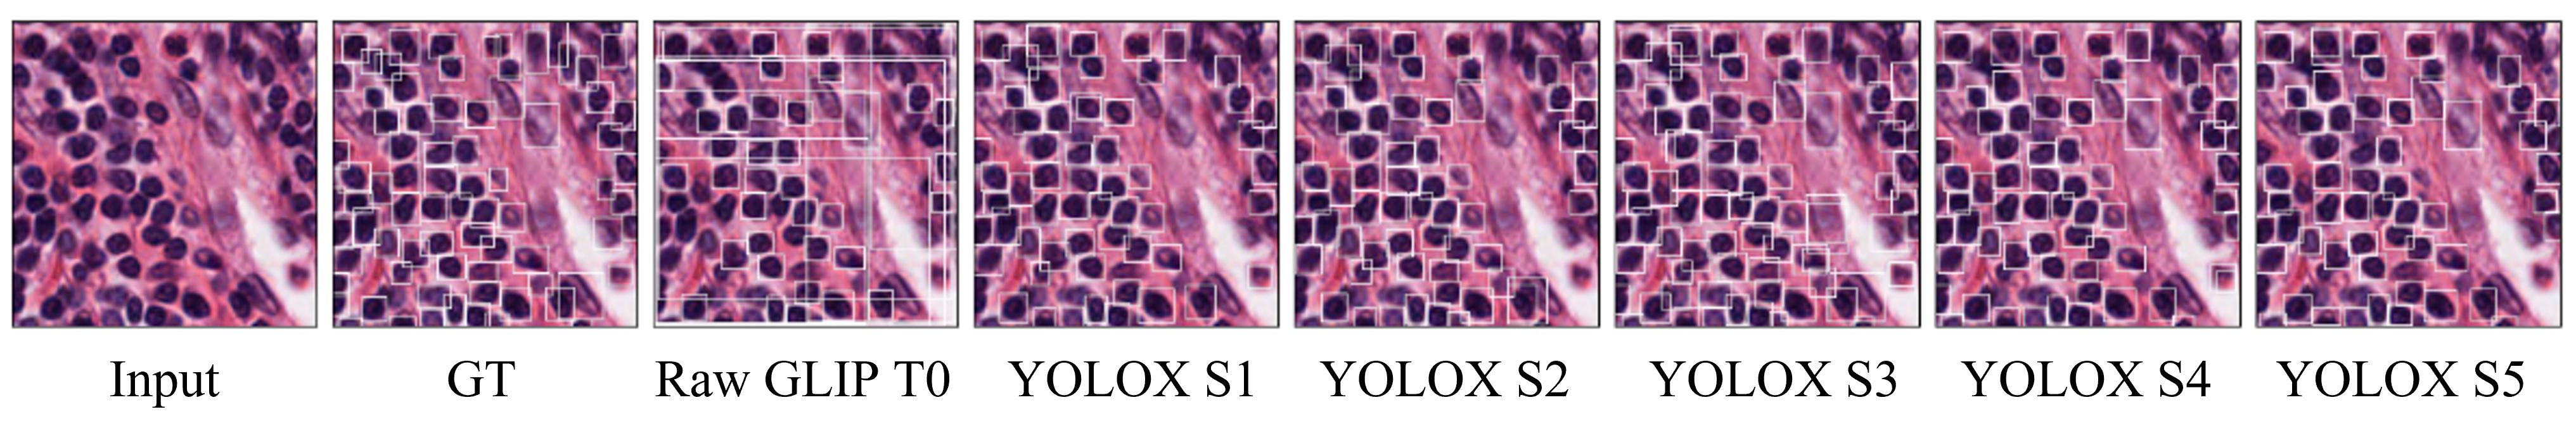
\includegraphics[width=\textwidth]{chapters/PAPERS/glip_miccai_camera_ready_supplement/self-training.png}
  \caption{MICCAI 工作中自训练策略带来的增益示意。图中展示了模型从初始零样本预测到伪标签自适配后的性能变化趋势与案例差异。}
  \label{fig:miccai_selftrain}
\end{figure}

\section{实验结果与讨论}
根据已发表工作，本章方法表明：通过自动属性提示和自训练，视觉语言预训练模型可以在没有专门检测标注的情况下，获得可用的细胞核检测能力。

\section{本章创新点总结}
本章的主要创新点体现在：第一，提出自动属性提示机制，使视觉语言模型能够在医学对象语义不足场景中获得更强提示能力；第二，将零样本视觉语言检测与自训练结合，实现从开放词汇识别到目标域适配的闭环；第三，验证了视觉语言预训练模型在医学检测中不仅可作为概念性工具，而且可作为实际有效的无标注检测入口。

\section{本章小结}
本章围绕零样本细胞核检测问题，提出自动属性提示与自训练联合框架，说明在缺少专门检测标注时，视觉语言模型依然可以通过语义构造和目标域反馈形成可用检测能力。
